\documentclass[../tesis_main.tex]{subfiles}


\chapter{Resultados y conclusiones}
En esta sección analizaremos los resultados obtenidos al probar el algoritmo RANSAC para encontrar planos modificando el numero de iteraciones. Observaremos el comportamiento del error y el tiempo de ejecución a fin de encontar el número óptimo de iteraciones para este algoritmo.\\

	El proceso para el análisis de datos fue el siguiente:se propuso un modelo de plano conocido por el usuario. Dicho modelo se obtuvo a partir del conocimiento de la altura del plano en este caso una mesa. Posteriormente se cuatificó la cantidad de puntos que entraban en este modelo ideal y se tomó como base para la medición de errores. Continuando con el procedimiento se modificó el algoritmo para realizar un número determinado de iteraciones (600, 200, 100, 50, 30, 24 y 20) y se midió el error relativo y el tiempo de ejecición, en cada uno de estos procedimientos.\\

	Para probar el algoritmo con 600 iteraciones se tomaron 50 muestras los resultados se puden observar en la siguiente gráfica.\\


	\begin{figure}[H]
		\begin{center}
		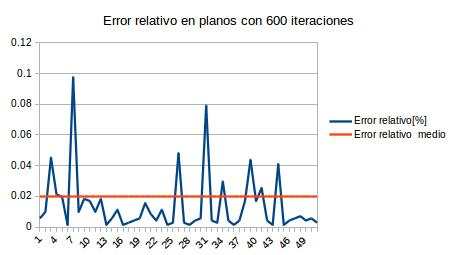
\includegraphics[width=10.5cm, height=3.4cm]{/600_errRel.jpg}	
		\caption{Segmentación de un objeto y sus correspondientes ejes principales (rojo).}

		\end{center}
	\end{figure}

	\begin{figure}[H]
		\begin{center}
		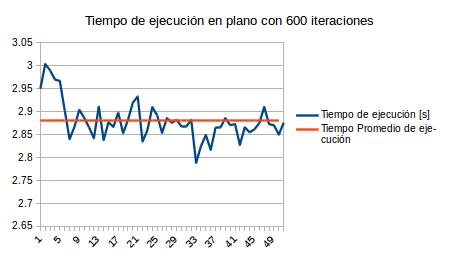
\includegraphics[width=12.5cm, height=6.0cm]{/600_timeExec.jpg}
		\caption{Segmentación de un objeto y sus correspondientes ejes principales (rojo).}
		\end{center}
	\end{figure}

	Se tomaron 50 muestras para el algoritmo modificado con 200 iteraciones. los resultados se puden observar en la siguiente gráfica.\\

	\begin{figure}[H]

		\begin{subfigure}[h]{.5\textwidth}
		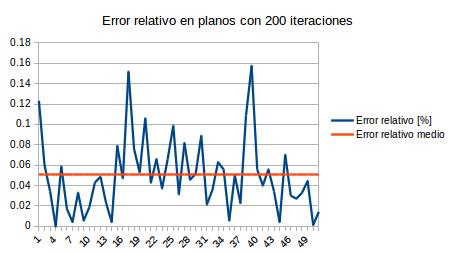
\includegraphics[width=8.5cm, height=5.0cm]{/200_errRel.jpg}	
		\end{subfigure}%
		\begin{subfigure}[h]{.5\textwidth}
		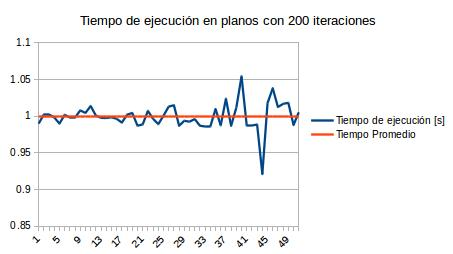
\includegraphics[width=8.5cm, height=5.0cm]{/200_timeExec.jpg}
		\end{subfigure}
	
	\caption{Segmentación de un objeto y sus correspondientes ejes principales (rojo).}

	\end{figure}

	Se continuó con el mismo principio para el algoritmo modificado con 100, 50, 30, 24 y 20 iteraciones respectivamente. Los resultados se pueden observar en las gráficas anexadas a continuación.\\


	\begin{figure}[H]

		\begin{subfigure}[h]{.5\textwidth}
		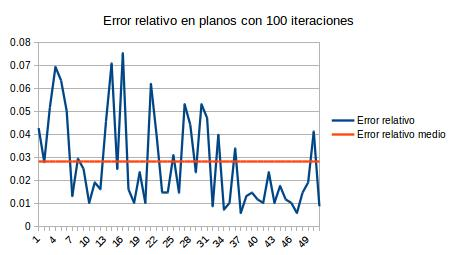
\includegraphics[width=8.5cm, height=5.0cm]{/100_errRel.jpg}	
		\end{subfigure}%
		\begin{subfigure}[h]{.5\textwidth}
		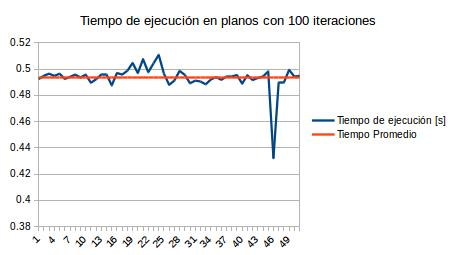
\includegraphics[width=8.5cm, height=5.0cm]{/100_timeExec.jpg}
		\end{subfigure}
	
	\caption{Segmentación de un objeto y sus correspondientes ejes principales (rojo).}

	\end{figure}

	\begin{figure}[H]

		\begin{subfigure}[h]{.5\textwidth}
		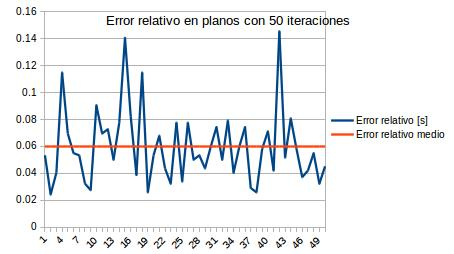
\includegraphics[width=8.5cm, height=5.0cm]{/50_errRel.jpg}	
		\end{subfigure}%
		\begin{subfigure}[h]{.5\textwidth}
		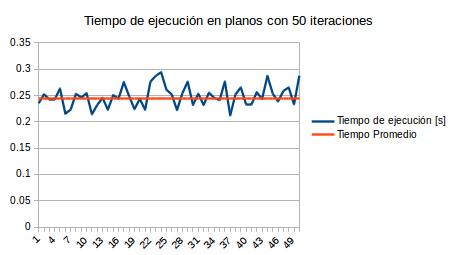
\includegraphics[width=8.5cm, height=5.0cm]{/50_timeExec.jpg}
		\end{subfigure}
	
	\caption{Segmentación de un objeto y sus correspondientes ejes principales (rojo).}

	\end{figure}

	\begin{figure}[H]

		\begin{subfigure}[h]{.5\textwidth}
		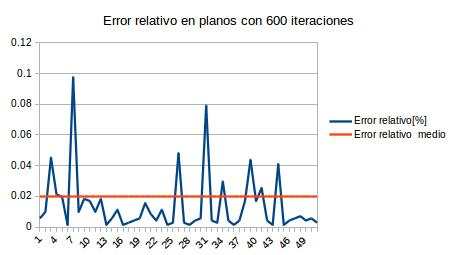
\includegraphics[width=8.5cm, height=5.0cm]{/600_errRel.jpg}	
		\end{subfigure}%
		\begin{subfigure}[h]{.5\textwidth}
		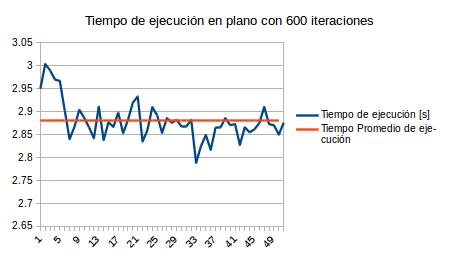
\includegraphics[width=8.5cm, height=5.0cm]{/600_timeExec.jpg}
		\end{subfigure}
	
	\caption{Segmentación de un objeto y sus correspondientes ejes principales (rojo).}

	\end{figure}

	\begin{figure}[ht!]

		\begin{subfigure}[h]{.5\textwidth}
		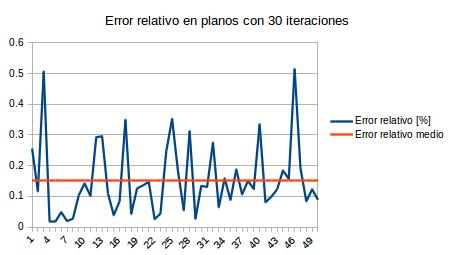
\includegraphics[width=8.5cm, height=5.0cm]{/30_errRel.jpg}	
		\end{subfigure}%
		\begin{subfigure}[h]{.5\textwidth}
		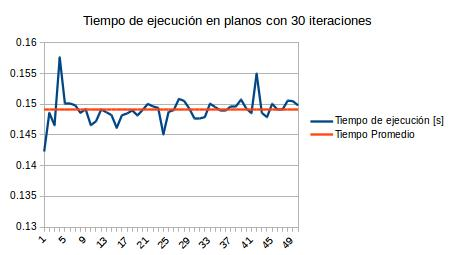
\includegraphics[width=8.5cm, height=5.0cm]{/30_timeExec.jpg}
		\end{subfigure}
	
	\caption{Segmentación de un objeto y sus correspondientes ejes principales (rojo).}

	\end{figure}

	\begin{figure}[H]

		\begin{subfigure}[h]{.5\textwidth}
		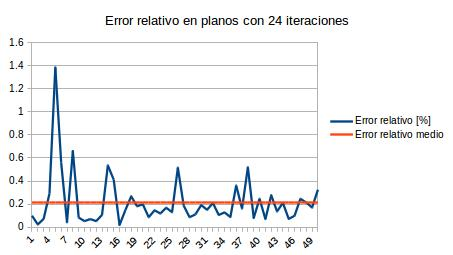
\includegraphics[width=8.5cm, height=5.0cm]{/24_errRel.jpg}	
		\end{subfigure}%
		\begin{subfigure}[h]{.5\textwidth}
		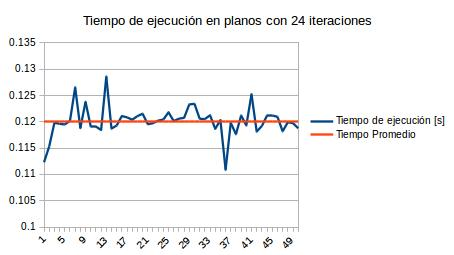
\includegraphics[width=8.5cm, height=5.0cm]{/24_timeExec.jpg}
		\end{subfigure}
	
	\caption{Segmentación de un objeto y sus correspondientes ejes principales (rojo).}

	\end{figure}

	\begin{figure}[H]

		\begin{subfigure}[h]{.5\textwidth}
		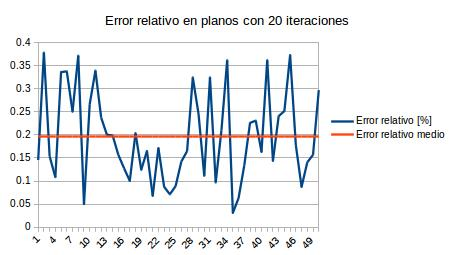
\includegraphics[width=8.5cm, height=5.0cm]{/20_errRel.jpg}	
		\end{subfigure}%
		\begin{subfigure}[h]{.5\textwidth}
		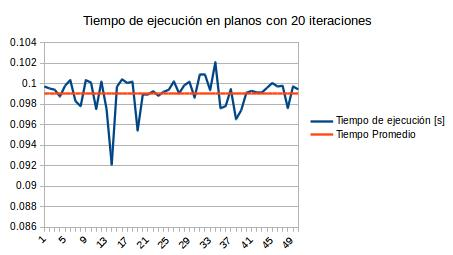
\includegraphics[width=8.5cm, height=5.0cm]{/20_timeExec.jpg}
		\end{subfigure}
	
	\caption{Segmentación de un objeto y sus correspondientes ejes principales (rojo).}

	\end{figure}

	Una vez que se obtuvo la información parcial de cada uno de estos eventos se realizó una tabla extra que agrupa la información del timepo de ejecución promedio y el error relativo promedio contra el número de iteraciones del algoritmo. Se obtuvo la siguiente gráfica.\\

	\begin{figure}[H]

		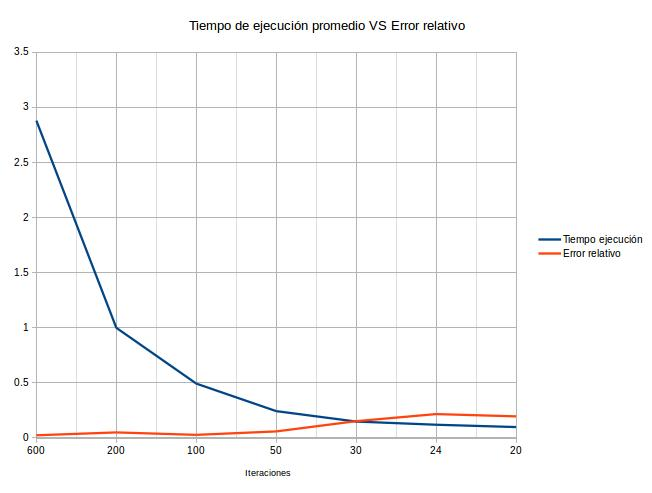
\includegraphics[width=14.5cm, height=8.0cm]{/timeExec_errRel.jpg}
		\caption{Segmentación de un objeto y sus correspondientes ejes principales (rojo).}

	\end{figure}


	Como podemos observar en la tabla 4.10 el error relativo presenta un incremento conforme se dismuye el número de iteraciones en el algoritmo. El tiempo de ejecución por su parte muestra un decremento conforme el número de iteraciones disminuye. Dado este comportamiento de ambos parámetros resulta dificil encontrar un punto de equilibrio entre estas dos unidades de medición. Sin embargo observamos que tanto el error relativo como el tiempo de ejecución llegan a un valor estable, a partir del cual no aumentan o disminuyen significativamente. La gráfica 4.10 nos sugiere que este punto está en un número de iteraciones entre 30 y 24.\\ 




%%%%%%%%%%%%%%%%%%%%%%%%%%%%%%%%%%%%%%%%%%%%%%%%%%%%%%%%%%%%
%%%%%%%%%		Conclusiones           %%%%%%%%%%%%%%%%%%%%%
%% \chapter{Conclusiones} 
	Partiendo de la información obtenida de los resultados podemos concluir que un algoritmo RANSAC con un humbral de 0.5 [cm] y un número de iteraciones entre 24 y 30 nos ayudará a encontrar la ecuación de un plano así como una lista de puntos pertenecientes al mismo. Esta primera parte del desarrollo permitió desarrrolar un algoritmo que no presentara un tiempo excesivo de ejecución de manera inecesaria. \\

	Una vez que se estuvo seguros que el algoritmo RANSAC funcionaba de manera aceptable se continuó a probar la extracción de objetos sobre el plano.

